% CVPR 2022 Paper Template
% based on the CVPR template provided by Ming-Ming Cheng (https://github.com/MCG-NKU/CVPR_Template)
% modified and extended by Stefan Roth (stefan.roth@NOSPAMtu-darmstadt.de)

\documentclass[10pt,twocolumn,letterpaper]{article}

%%%%%%%%% PAPER TYPE  - PLEASE UPDATE FOR FINAL VERSION
%\usepackage[review]{cvpr}      % To produce the REVIEW version
\usepackage{cvpr}              % To produce the CAMERA-READY version
%\usepackage[pagenumbers]{cvpr} % To force page numbers, e.g. for an arXiv version

% Include other packages here, before hyperref.
\usepackage{graphicx}
\usepackage{amsmath}
\usepackage{amssymb}
\usepackage{booktabs}
\usepackage{breqn}


% It is strongly recommended to use hyperref, especially for the review version.
% hyperref with option pagebackref eases the reviewers' job.
% Please disable hyperref *only* if you encounter grave issues, e.g. with the
% file validation for the camera-ready version.
%
% If you comment hyperref and then uncomment it, you should delete
% ReviewTempalte.aux before re-running LaTeX.
% (Or just hit 'q' on the first LaTeX run, let it finish, and you
%  should be clear).
\usepackage[pagebackref,breaklinks,colorlinks]{hyperref}


% Support for easy cross-referencing
\usepackage[capitalize]{cleveref}
\crefname{section}{Sec.}{Secs.}
\Crefname{section}{Section}{Sections}
\Crefname{table}{Table}{Tables}
\crefname{table}{Tab.}{Tabs.}


%%%%%%%%% PAPER ID  - PLEASE UPDATE
\def\cvprPaperID{*****} % *** Enter the CVPR Paper ID here
\def\confName{CVPR}
\def\confYear{2022}


\begin{document}

%%%%%%%%% TITLE - PLEASE UPDATE
\title{Vision Systems Project Report\\
Project Title: Understanding similarity of Saliency Maps between NR IQA Models and Vision Classification Models}

\author{Krishna Srikar Durbha\\
{\tt\small krishna.durbha@utexas.edu}
% For a paper whose authors are all at the same institution,
% omit the following lines up until the closing ``}''.
% Additional authors and addresses can be added with ``\and'',
% just like the second author.
% To save space, use either the email address or home page, not both
}
\maketitle

%%%%%%%%% ABSTRACT
\begin{abstract}
In recent years, convolutional neural networks (CNNs) have been copiously applied in various image and video processing problems giving state-of-the-art results close to human-level performance. They are used for real-time scenarios like quality assessment, object detection, autonomous navigation, satellite imaging, etc. But for the SOTA (state-of-the-art) models to maintain their performance, they need images/videos to follow a distribution on which they are trained. Any example that lies outside this distribution might reduce the model's performance. In this report, we try to understand the similarities or differences in perception of the basic computer vision image classification model and humans.
We try to understand the correlation between them by comparing the performance of vision models with image quality rated by no-reference image quality assessment algorithms, which are trained to approximate human judgements.
\end{abstract}

%%%%%%%%% BODY TEXT

\section{Introduction}
\label{sec:intro}
Convolutional neural networks (CNNs) are a class of deep neural networks that have become prominent in various image and video processing tasks. They perform incredibly in extracting spatial features of visual data of images and videos. CNN can learn complex features required from images for recognition, detection, segmentation, and retrieval using a hierarchy of trainable filters and feature pooling operations. They have proven to be successful in tasks related to image quality assessment \cite{PaQ-2-PiQ}, and computer vision \cite{ImageNet} give state-of-the-art results close to the performance of humans.\\

Quality can be considered as the accuracy with which information is contained. In the case of images which are signals, the techniques used to capture, the accuracy of detail, colour, contrast, luminance etc., become various factors in determining the quality of the image.\\

Image quality assessment algorithms are used in rating the quality of images and are divided into three categories.
\begin{itemize}
    \setlength\itemsep{0.001em}
    \item Reference IQA algorithms need a reference and distorted images to estimate quality.
    \item Reduced IQA algorithms: Need less information about reference image and require the entire distorted image to estimate quality. 
    \item No Reference IQA algorithms: Need no reference image at all. They only need a distorted image to estimate quality.
\end{itemize}
NR IQA algorithms are trained on ratings of various images collected from humans. Many human studies have been conducted to create massive datasets consisting of subjective image evaluations. Over the years, NR IQA algorithms used NSS (Natural Scene Statistics), which is an important field of vision science \cite{NSS} as their base to develop various algorithms  \cite{DIIVINE}, \cite{BRISUQE}, \cite{NIQE} etc. Recently with the surge of deep learning and its ability to extract features and create better approximations, these NR IQA algorithms started using CNNs in their algorithms \cite{PaQ-2-PiQ} etc.\\

CNNs also played a major in the rise of computer vision algorithms. Every new model or algorithm is developed to achieve state-or-the-art results on major computer vision datasets like ImageNet, Kinetics-700, MS Coco, Open Images etc., on various tasks like classification, segmentation, detection, generation, compression etc. CNN models like \cite{InceptionNet}, \cite{ResNet} etc. reached state-of-the-art on these standard datasets with their performance very close to humans. To understand what these high-accuracy models are learning and to understand these models better, techniques like Vanilla Gradients, Grad-CAM, Grad-CAM++, LIME etc., have been developed to understand the perception of these computer vision models. These are explainable AI techniques or Pixel attribution methods that highlight the relevant pixels for image classification by a neural network.

\begin{figure}[!ht]
	\centering
	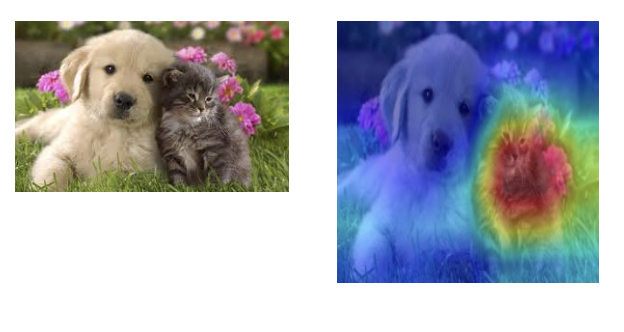
\includegraphics[width=\columnwidth]{Images/Grad-CAM.png}
	\caption{Pixel Attribution Map using Grad-CAM of ResNet50 detecting a `cat'.}
\end{figure}

%------------------------------------------------------------------------

\section{Problem Statement}
\label{sec:problem}
The term perception is very different for humans and computers. Understanding a scene comes naturally to us without any effort, but for computers, there is no such thing as conscious; it is just a bunch of filters leading to a prediction. The distortions in images are usually an aspect of electronic noise produced by an image sensor or the circuitry of a scanner or digital camera. These disturbances occur naturally while capturing or transmitting, or saving an image. These distortions are visible to the human eye. They can also be affected by the brightness, contrast, saturation, settings, zooming, weather conditions, compression etc.\\

In this report, we will observe if there is a correlation between the performance of the image classification model and quality rating given by an NR IQA algorithm not only in terms of accuracy but also plotting saliency maps and local patch qualities, respectively. As NR-IQA models are trained on human judgements/perception, they help to understand the similarity in the perception of an image as humans rate it and the classification model while they classify it.\\

As a part of the experiment, we will use images from a dataset rated as good by a no-reference IQA algorithm. As NR-IQA algorithms are the closest approximation of human ratings, they should help us understand how humans would rate images. Then, by splitting the dataset into train and validation sets, we will train an image classification model on the training set and validate its performance on the validation set with different types of natural distortions and various levels. We are training a classification model on high-quality images to understand its perception of distortions wrt humans. We then generate the saliency maps from the image classification model and compare them with the patch-wise quality estimate obtained from the NR-IQA model.

%------------------------------------------------------------------------

\section{Literature}
\label{section:literature}

Paper \cite{DodgeK16} discuss how the quality of the image affects the performance of neural networks. It shows that when a model is trained on uncorrupted images, its performance is affected when tested on images with distortions like Blur, Noise, Contrast, JPEG and JPEG 2000. Also, the performance decreases with the extent of corruption. This follows that a data shift affects the performance of a model trained in a distribution. The paper concludes with the possibility that training models with low-quality images might lead to better performance on low-quality images but also increases the risk of misclassification on high-quality images.\\

One of the key points to note is that adding noise to images during training is one of the data augmentation techniques. So, training the model on noisy images should help create robust models, but in fact, it is not the case. Paper \cite{akbiyik2020data} discuss the correlation between the level of noise that needed to be added to an image to create robust images and the structural similarity index metric. It concludes by saying that to create a robust model against particular noise while maintaining the model's performance, the amount of degradation that should be applied should result around a quality estimate of 0.8 MS-SSIM.\\

The above literature provides an understanding that there is a correlation between the quality estimate and the performance of a classification vision model. As a reference image might only be available some of the time, we considered no reference image quality estimation techniques to rate the quality of images.

%------------------------------------------------------------------------

\section{Approach}
\label{section:approach}
\subsection{Dataset and Data Preprocessing}
As a part of our experiment, we shall use the mit-indoor-scenes dataset \cite{mit-indoor-scenes}. The dataset consists of 67 indoor scene categories with 15620 images. Among all the images, we get the images which are rated `Good' or `Excellent' by our NR IQA model among `Bad', `Poor', `Fair', `Good' and `Excellent'. The quality of the dataset is as follows:
\begin{figure}[!ht]
    \centering
    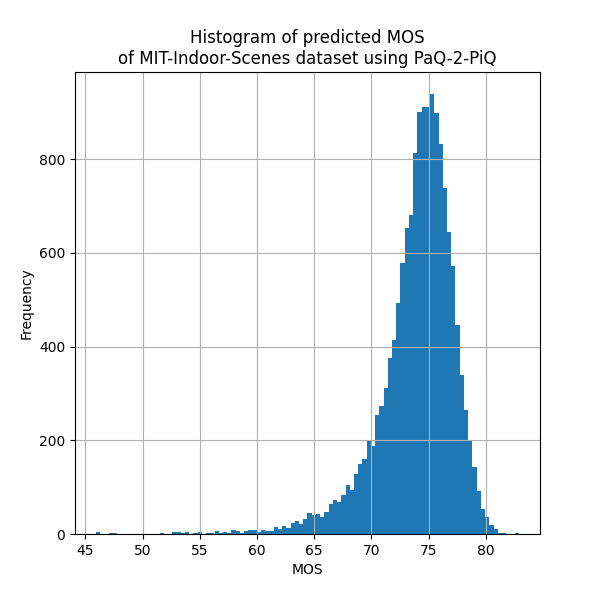
\includegraphics[width=\columnwidth]{Images/MOS_Histogram.png}
    \caption{MOS of images in the dataset}
\end{figure}
\begin{figure}[!ht]
    \centering
    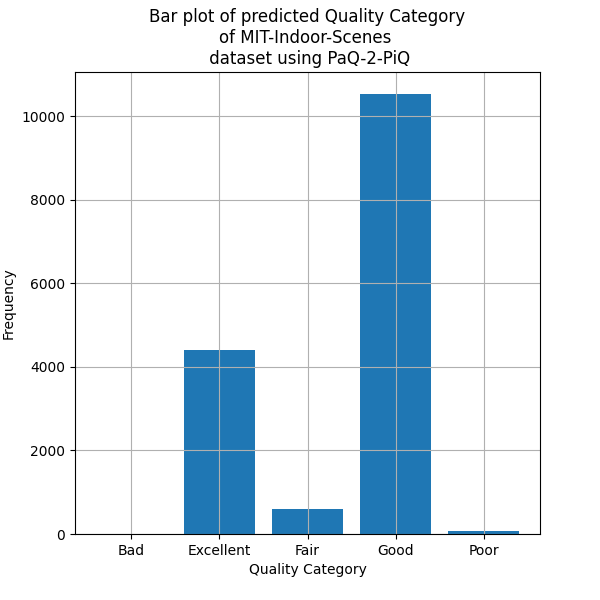
\includegraphics[width=\columnwidth]{Images/Quality_Category_Histogram.png}
    \caption{Quality category of images in the dataset}
\end{figure}\\

We split the rated images into 80-20 as training and validation sets. We train our image classification models on the training set and evaluate them on the validation set.
We will observe the model's performance in terms of accuracy and attribution maps on various corruptions like `brightness', `contrast', `jpeg_compression', and `saturate' with severity levels \{1,2\}. We use the term severity to explain how strongly the image is distorted. For further reference check \href{https://github.com/bethgelab/imagecorruptions}{ImageCorruptions}\\

\subsection{Models}
We use the PaQ-2-PiQ model as a no-reference image quality assessment algorithm for rating images. The PaQ-2-PiQ model has three different variations. In the model, we use the RoIPool layer similar to Fast-RCNN, which allows flexibility to train both patch and picture-sized scales. It has a ResNet18 model as its backbone, followed by RoIPool and two fully connected layers. In this paper, whenever we refer to the NR-IQA PaQ-2-PiQ model, we refer to the model with only the RoIPool layer without feedback. We will use the ResNet18 model with the last two layers modified to maintain consistency with the PaQ-2-PiQ model as a classification model. 
%------------------------------------------------------------------------

\section{Results}
Consider the image below. We are going to show the variation in attribution maps of both ResNet and Paq-2PiQ for different distortions and different levels.
\begin{figure}[!ht]
    \centering
    \includegraphics[width=.49\columnwidth]{Images/test_images/severity=-1/buffet.png}
    \hfill
    \includegraphics[width=.49\columnwidth]{Images/test_images/severity=0/buffet.png}\hfill
    \\[\smallskipamount]
    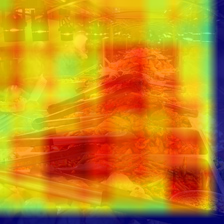
\includegraphics[width=.49\columnwidth]{Images/saliency_maps/paq2piq/severity=0/buffet.png}\hfill
    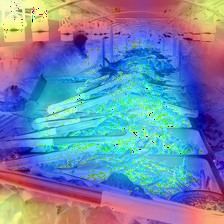
\includegraphics[width=.49\columnwidth]{Images/saliency_maps/resnet18/severity=0/buffet.png}\hfill
    \caption{First row: Original image and center cropped version of the original one, respectively. The quality estimations from PaQ-2-PiQ are 76.75, 76.75, respectively. Second row: Attribution maps from PaQ-2-PiQ and ResNet, respectively on the cropped original image.}
\end{figure}

Distortions are first added to the original image; then the distorted image is center-cropped to shape (224,224). Images are cropped instead of resized to maintain originality as we perform the quality estimation.\\

In the figures below; In the first row, the left one is cropped original image and the right one is cropped distorted image with a particular similarity; In the second row, the left image is the local patch quality of the cropped distorted image from PaQ-2-PiQ and the right image is attribution map of the cropped distorted image from ResNet. We will also describe the quality ratings of original and distorted images along with severity.\\

PaQ-2-PiQ for NR-IQA and ResNet for classification have the same backbone model as mentioned. We chose such models to clearly observe the difference in image perception of models with two different goals. The goal of PaQ-2-PiQ is to estimate the image's quality, whereas the goal of ResNet is to classify it. Due to their inherited same backbone structure, the areas they tend to focus on without distortions with be very close. But the benefit is we get to understand the change in their perception of distortions in images.

\subsection{Brightness Distortion}
\begin{figure}[!ht]
	\centering
	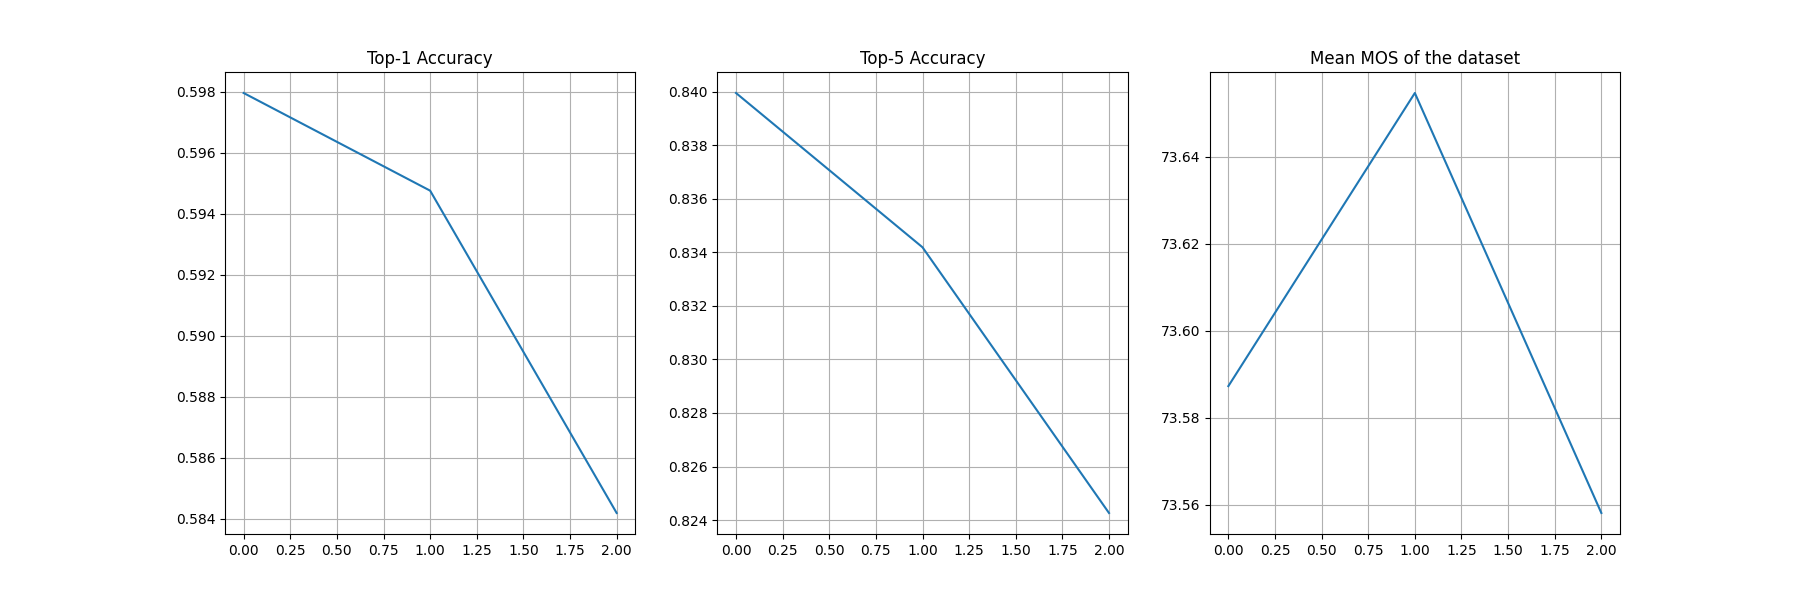
\includegraphics[width=1.\columnwidth]{Images/brightness.png}
	\caption{The figure show the change in Top@1, Top@5 Accuracies and Mean MOS on the validation dataset by changing severity of brightness corruption.}
\end{figure}

\begin{figure}[!ht]
	\includegraphics[width=.49\columnwidth]{Images/test_images/severity=0/buffet.png}\hfill
	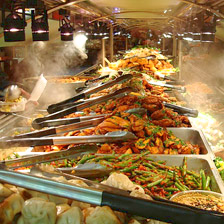
\includegraphics[width=.49\columnwidth]{Images/test_images/severity=1/brightness/buffet.png}\hfill
	\\[\smallskipamount]
    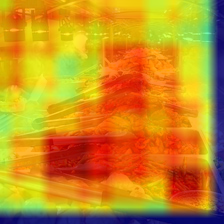
\includegraphics[width=.49\columnwidth]{Images/saliency_maps/paq2piq/severity=1/brightness/buffet.png}\hfill
	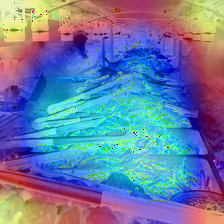
\includegraphics[width=.49\columnwidth]{Images/saliency_maps/resnet18/severity=1/brightness/buffet.png}\hfill
    \caption{Brightness Severity = 1. The quality estimations from PaQ-2-PiQ are 76.75, 76.97 respectively (left to right).}
\end{figure}

\begin{figure}[!ht]
	\includegraphics[width=.49\columnwidth]{Images/test_images/severity=0/buffet.png}\hfill
	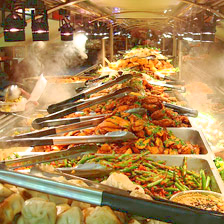
\includegraphics[width=.49\columnwidth]{Images/test_images/severity=2/brightness/buffet.png}\hfill
	\\[\smallskipamount]
    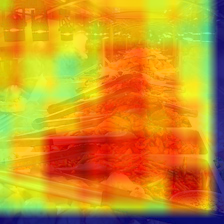
\includegraphics[width=.49\columnwidth]{Images/saliency_maps/paq2piq/severity=2/brightness/buffet.png}\hfill
	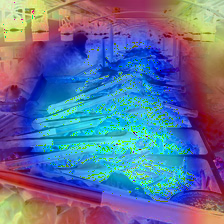
\includegraphics[width=.49\columnwidth]{Images/saliency_maps/resnet18/severity=2/brightness/buffet.png}\hfill
	\caption{Brightness Severity = 2. The quality estimations from PaQ-2-PiQ are 76.75, 76.66 respectively (left to right).}
\end{figure}

The variation in accuracy and MOS wrt brightness distortion are minor. This is also reflected in both quality maps and attribution maps. Also, the change in brightness is causing a shift in the quality map, particularly the quality of certain patches. The slight differences can be seen in the quality map's top left and central areas. This difference can also be observed inside the blue region of the attribution map.

\subsection{Contrast Distortion}
\begin{figure}[!ht]
	\centering
	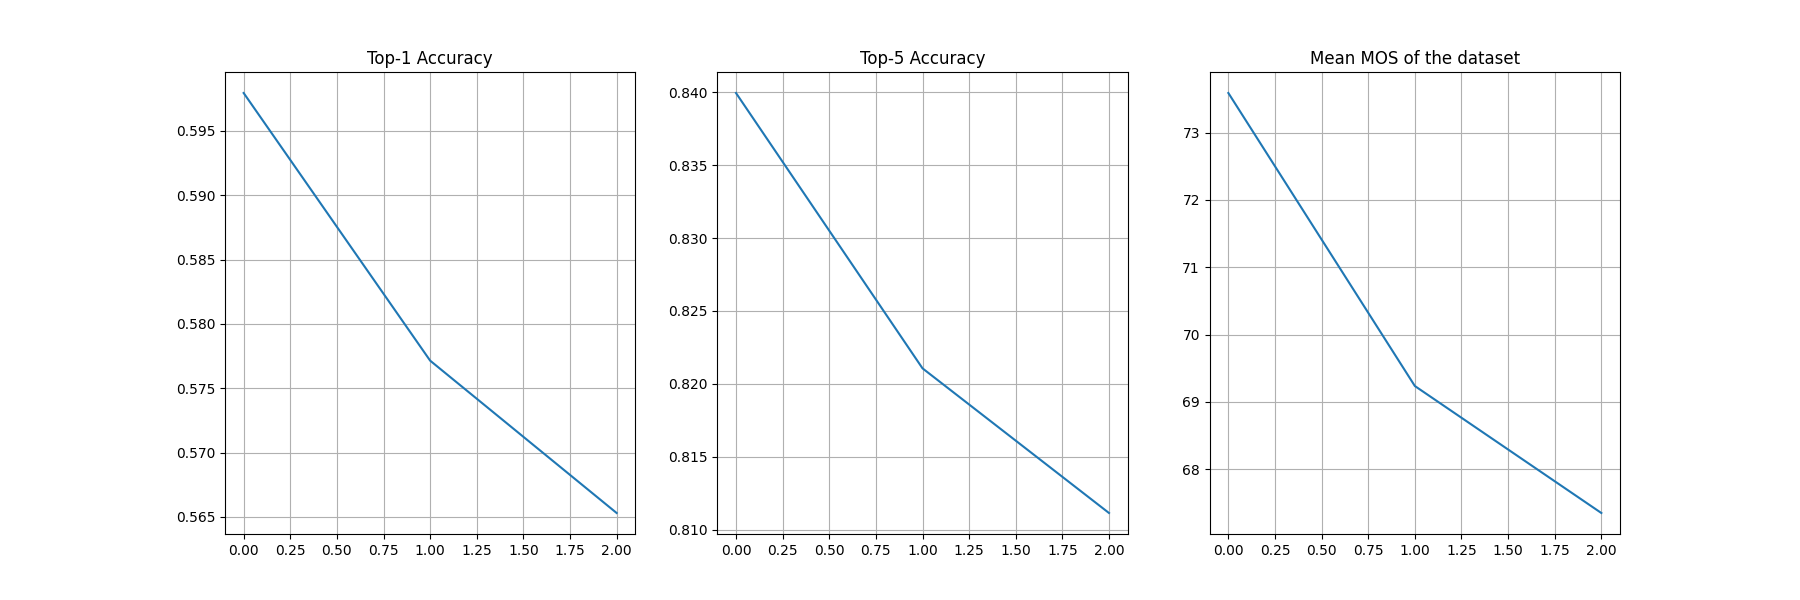
\includegraphics[width=1.\columnwidth]{Images/contrast.png}
	\caption{The figure show the change in Top@1, Top@5 Accuracies and Mean MOS on the validation dataset by changing severity of contrast corruption.}
\end{figure}

\begin{figure}[!ht]
	\includegraphics[width=.49\columnwidth]{Images/test_images/severity=0/buffet.png}\hfill
	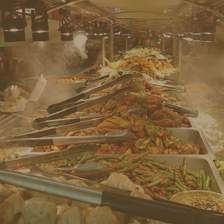
\includegraphics[width=.49\columnwidth]{Images/test_images/severity=1/contrast/buffet.png}\hfill
	\\[\smallskipamount]
    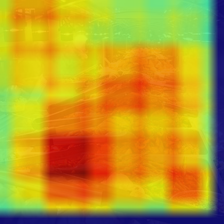
\includegraphics[width=.49\columnwidth]{Images/saliency_maps/paq2piq/severity=1/contrast/buffet.png}\hfill
	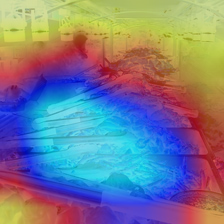
\includegraphics[width=.49\columnwidth]{Images/saliency_maps/resnet18/severity=1/contrast/buffet.png}\hfill
	\caption{Contrast Severity = 1. The quality estimations from PaQ-2-PiQ are 76.75, 71.19 respectively (left to right).}
\end{figure}

\begin{figure}[!ht]
	\includegraphics[width=.49\columnwidth]{Images/test_images/severity=0/buffet.png}\hfill
	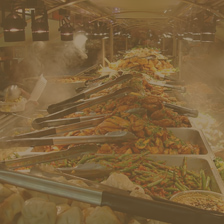
\includegraphics[width=.49\columnwidth]{Images/test_images/severity=2/contrast/buffet.png}\hfill
	\\[\smallskipamount]
    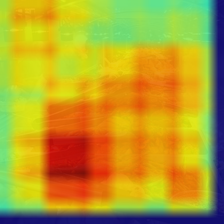
\includegraphics[width=.49\columnwidth]{Images/saliency_maps/paq2piq/severity=2/contrast/buffet.png}\hfill
	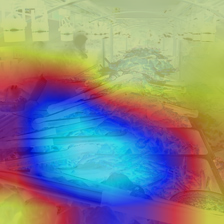
\includegraphics[width=.49\columnwidth]{Images/saliency_maps/resnet18/severity=2/contrast/buffet.png}\hfill
	\caption{Constrast Severity = 2. The quality estimations from PaQ-2-PiQ are 76.75, 70.31 respectively (left to right).}
\end{figure}

The variation in accuracy and MOS wrt change in contrast distortion is very significant. This is also reflected in both quality maps and attribution maps. The contrast distortion has shifted the focus of attribution maps. The area where the ResNet lost its focus is also where the image quality is low.

\subsection{JPEG Compression Distortion}
\begin{figure}[!ht]
	\centering
	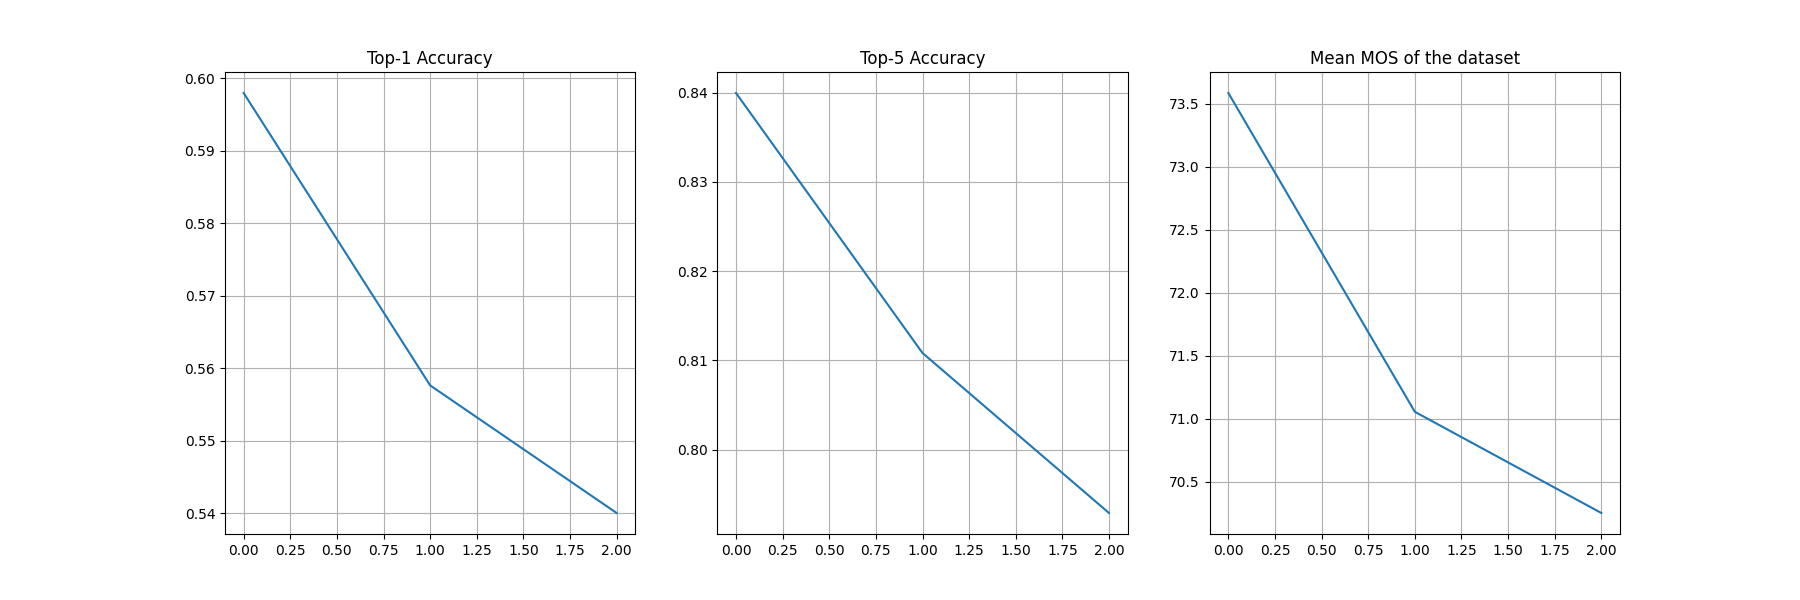
\includegraphics[width=1.\columnwidth]{Images/jpeg_compression.png}
	\caption{The figure show the change in Top@1, Top@5 Accuracies and Mean MOS on the validation dataset by changing severity of jpeg compression corruption.}
\end{figure}

\begin{figure}[!ht]
	\includegraphics[width=.49\columnwidth]{Images/test_images/severity=0/buffet.png}\hfill
	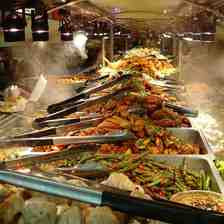
\includegraphics[width=.49\columnwidth]{Images/test_images/severity=1/jpeg_compression/buffet.png}\hfill
	\\[\smallskipamount]
    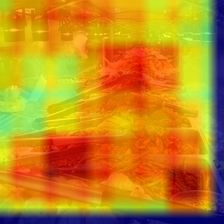
\includegraphics[width=.49\columnwidth]{Images/saliency_maps/paq2piq/severity=1/jpeg_compression/buffet.png}\hfill
	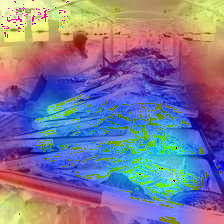
\includegraphics[width=.49\columnwidth]{Images/saliency_maps/resnet18/severity=1/jpeg_compression/buffet.png}\hfill
	\caption{JPEG Compression Severity = 1. The quality estimations from PaQ-2-PiQ are 76.75, 72.19 respectively (left to right).}
\end{figure}

\begin{figure}[!ht]
	\includegraphics[width=.49\columnwidth]{Images/test_images/severity=0/buffet.png}\hfill
	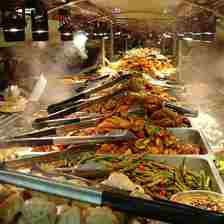
\includegraphics[width=.49\columnwidth]{Images/test_images/severity=2/jpeg_compression/buffet.png}\hfill
	\\[\smallskipamount]
    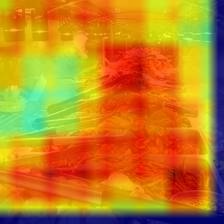
\includegraphics[width=.49\columnwidth]{Images/saliency_maps/paq2piq/severity=2/jpeg_compression/buffet.png}\hfill
	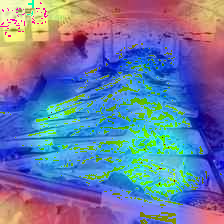
\includegraphics[width=.49\columnwidth]{Images/saliency_maps/resnet18/severity=2/jpeg_compression/buffet.png}\hfill
	\caption{JPEG Compression Severity = 2. The quality estimations from PaQ-2-PiQ are 76.75, 71.58 respectively (left to right).}
\end{figure}

The variation in accuracy and MOS wrt change in jpeg compression distortion is very significant but unique. From the attribution maps, it can be understood that the JPEG compression didn't change the area the ResNet focuses on but has changed the importance of those areas. A similar goes for the case of quality maps; it has affected the quality of individual patches and the quality of the entire image, but the areas considered for overall quality prediction are not changed.

\subsection{Saturate Distortion}
\begin{figure}[!ht]
	\centering
	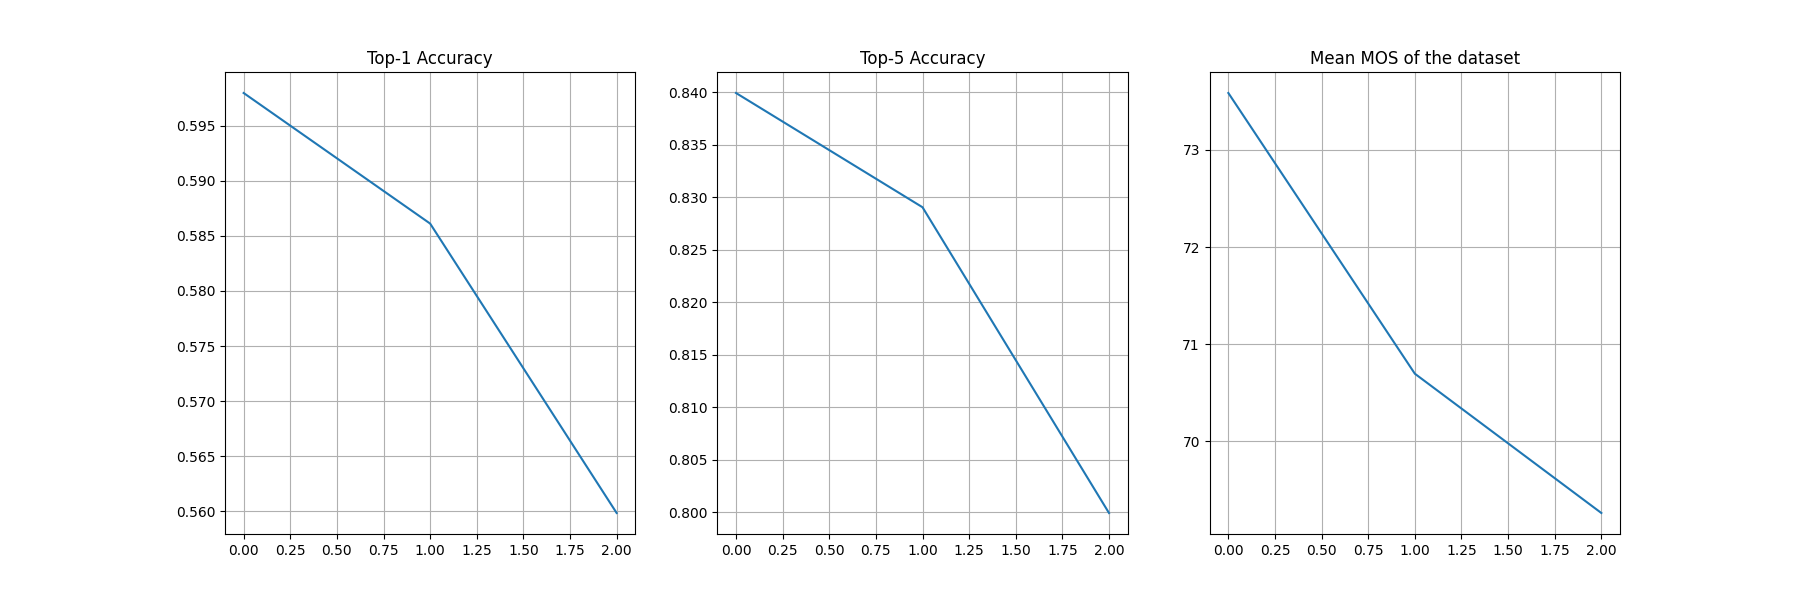
\includegraphics[width=1.\columnwidth]{Images/saturate.png}
	\caption{The figure show the change in Top@1, Top@5 Accuracies and Mean MOS on the validation dataset by changing severity of saturate corruption.}
\end{figure}

\begin{figure}[!ht]
	\includegraphics[width=.49\columnwidth]{Images/test_images/severity=0/buffet.png}\hfill
	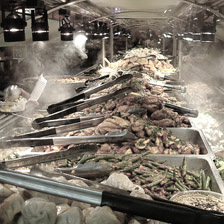
\includegraphics[width=.49\columnwidth]{Images/test_images/severity=1/saturate/buffet.png}\hfill
	\\[\smallskipamount]
    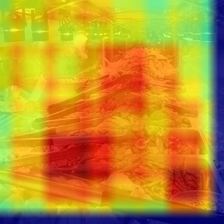
\includegraphics[width=.49\columnwidth]{Images/saliency_maps/paq2piq/severity=1/saturate/buffet.png}\hfill
	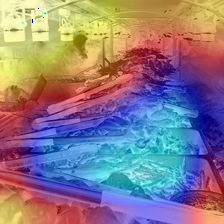
\includegraphics[width=.49\columnwidth]{Images/saliency_maps/resnet18/severity=1/saturate/buffet.png}\hfill
	\caption{Saturation Severity = 1. The quality estimations from PaQ-2-PiQ are 76.75, 72.73 respectively (left to right).}
\end{figure}

\begin{figure}[!ht]
	\includegraphics[width=.49\columnwidth]{Images/test_images/severity=0/buffet.png}\hfill
	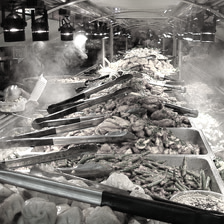
\includegraphics[width=.49\columnwidth]{Images/test_images/severity=2/saturate/buffet.png}\hfill
	\\[\smallskipamount]
    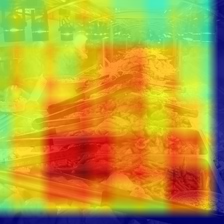
\includegraphics[width=.49\columnwidth]{Images/saliency_maps/paq2piq/severity=2/saturate/buffet.png}\hfill
	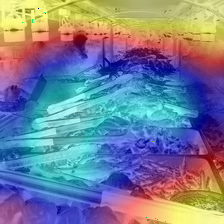
\includegraphics[width=.49\columnwidth]{Images/saliency_maps/resnet18/severity=2/saturate/buffet.png}\hfill
	\caption{Saturation Severity = 2. The quality estimations from PaQ-2-PiQ are 76.75, 70.6 respectively (left to right).}
\end{figure}

The variation in accuracy and MOS wrt change in the saturation level of distortion is significant. The effect of saturation is very peculiar. In this case, saturation reduces the quality of the patches making the quality estimate of the image lower. But in attribution maps, the effect is quality is reflected, but there is less similarity between the change in quality map and attribution map.

%-------------------------------------------------------------------------

\section{Conclusion}
Noise in an image causes performance degradation in classification models. While rating an image, humans observe various portions to rate the quality. PaQ-2-PiQ is an NR-IQA model that is trained on human ratings of patches and images. To understand the similarities of perception of humans and computer vision models, we 
have considered two models PaQ-2-PiQ for NR-IQA and ResNet, for classification with a similar backbone structure of ResNet18 but with two different goals. The change in MOS of the image rated using PaQ-2-PiQ seems to be related to the accuracy of the classification model. This can not be explained by the plots having the variation of accuracies and MOS but also the saliency/attribution maps. The quality maps from PaQ-2-PiQ and attribution maps are affected similarly due to distortions. So, one can understand that there is some correlation between how humans perceive images while rating them and how computers see images while classifying them.

%-------------------------------------------------------------------------

%%%%%%%%% REFERENCES
{\small
\bibliographystyle{ieee_fullname}
\bibliography{egbib.bib}
}


\end{document}